\documentclass[runningheads]{llncs}
\usepackage[T1]{fontenc}  

\usepackage{graphicx}
\graphicspath{{./figures/}}

\usepackage{float}
%\usepackage{etoolbox} 
\usepackage{amsmath}
\usepackage{amssymb}
\usepackage{booktabs} 
\usepackage{algorithm}
\usepackage{algpseudocode}
\usepackage{url} 
\usepackage{silence} 

\WarningFilter{latex}{Command \showhyphens has changed}
\WarningFilter{hyperref}{Token not allowed in a PDF string}
\WarningFilter{fancyhdr}{\headheight is too small}

\setlength{\textfloatsep}{6pt plus 1pt minus 2pt}
\setlength{\floatsep}{5pt plus 1pt minus 2pt}
\setlength{\intextsep}{6pt plus 1pt minus 2pt}
\setlength{\abovecaptionskip}{3pt}
\setlength{\belowcaptionskip}{0pt}
\setlength{\abovedisplayskip}{4pt plus 1pt minus 1pt}
\setlength{\belowdisplayskip}{4pt plus 1pt minus 1pt}
\setlength{\abovedisplayshortskip}{3pt plus 1pt minus 1pt}
\setlength{\belowdisplayshortskip}{3pt plus 1pt minus 1pt}
\setlength{\jot}{2pt}

%%%\AtBeginEnvironment{algorithmic}{\footnotesize}
%%\AtBeginEnvironment{algorithm}{\vspace{-4pt}}
%\AfterEndEnvironment{algorithm}{\vspace{-6pt}}

%
\begin{document}
    \title{Infrastructure-as-Code MLOps for Predictive Analytics}

    \author{Anonymous Author(s)}

    \authorrunning{Anonymous Author(s)}

    \institute{Affiliations withheld for double-blind review}

    %
    \maketitle
    \begin{abstract}
        Institutional predictive systems are hard to reproduce once ingestion, evaluation, deployment, and reporting are built as separate steps. We present an Infrastructure-as-Code MLOps workflow that binds those steps into one traceable pipeline: a deterministic adapter feeds PostgreSQL persistence, a blocked temporal evaluator chooses a forecasting model, and a schema-validated reporter emits auditable evidence, all run in containers and declared for Azure through Terraform. We evaluated it on a dataset of 87,073 administrative publication records from 2015--2023, aggregated into nine annual observations. Over three chronological folds, eight candidates were compared by mean absolute percentage error (MAPE) and fold instability; Naive and simple exponential smoothing tied for the best score, and parsimony kept Naive, which projected 15,229 records per year for 2024--2026 within an exploratory residual-calibrated 80\% interval of 9,541.5--20,916.5. Host and container runs agreed on every non-numeric field and, on the 45 numeric differences, stayed inside a declared absolute-or-relative tolerance, even though their full payload hashes diverged. The result is an auditable evidence contract that ties source identity, model-selection evidence, generated artifacts, and reporting outputs to a single reproducible execution.
        \keywords{reproducibility \and auditable evidence \and data provenance \and temporal cross-validation \and containerized workflows}
    \end{abstract}

    \section{Introduction}

        Machine-learning systems now inform forecasting and institutional decisions~\cite{ref26}, yet a prediction is only as trustworthy as the trail that documents how it was produced~\cite{ref22}. MLOps builds that trail by drawing data ingestion, model development, deployment, monitoring, and governance into a single traceable lifecycle whose reliability in production is itself an active concern~\cite{ref1,ref2,ref3,ref23}. Reproducibility then rests on keeping four things intact: the identity of the dataset, the conditions under which it ran, the evidence behind model selection, and the artifacts produced along the way.

        In practice these stages are often built and run in isolation. When they drift apart, the datasets, metrics, figures, and outputs produced in one environment stop matching those produced in another. Prior taxonomies and data-pipeline studies map the lifecycle and document how schema, quality, and provenance failures propagate downstream~\cite{ref4,ref5,ref6}, and data-centric perspectives treat data quality and governance as first-class pipeline concerns rather than afterthoughts~\cite{ref24}.

        Containerized and provenance-aware workflows have been proposed to preserve dependencies, runtime conditions, and processing records~\cite{ref4,ref5,ref7,ref8}; recent work captures end-to-end provenance across an ML pipeline~\cite{ref21}, and frameworks now support reproducible computational experiments across scientific domains~\cite{ref25}. Yet most of these efforts either target one platform capability or describe the lifecycle in the abstract, and what is still missing is a single contract that binds the identity of the data, the preprocessing decisions, the temporal evaluation, the artifacts these yield, and the comparison of results across environments.

        This paper designs and evaluates such a contract. Built as Infrastructure-as-Code, the workflow runs the whole path from a deterministic dataset adapter to auditable evidence generation inside containers, and declares its Azure counterpart through Terraform. Three questions frame the evaluation: do provenance records and scientific artifacts stay internally consistent (RQ1); are host and container executions numerically equivalent under a declared policy (RQ2); and which forecasting candidate is defensible for a nine-observation annual series under blocked temporal validation (RQ3).

        The case rests on 87,073 administrative publication records from 2015--2023, collapsed into nine annual observations, so the study speaks to traceability, evidence consistency, and tolerance-based reproducibility within a bounded setting rather than to forecasting accuracy at large. We deliberately set aside any claim of a new algorithm, a production-grade platform, continuous monitoring, or superior Azure performance. Figure~\ref{fig:workflow} traces the workflow from end to end.

        \begin{figure}
            \centering
            
\includegraphics[width=\textwidth]{fig1.png}
            \caption{End-to-end Infrastructure-as-Code MLOps workflow. Green, blue, and violet mark three stages: ingestion and persistence, evaluation and evidence generation, and reporting. The circular arrow marks a full, repeatable re-run.}
            \label{fig:workflow}
        \end{figure}
    \section{Methods}
        We built the artifact under design-science guidance, keeping its construction, evaluation, and communication transparent~\cite{ref9,ref10}. The work moved through the familiar design-science stages: naming the problem, fixing the solution objectives, designing and building the artifact, demonstrating it, and evaluating what it produced.

        \subsection{Architecture, Ingestion, and Evidence Contract}

            Six logical components make up the workflow: a dataset adapter, PostgreSQL persistence, a temporal evaluation engine, an evidence registry, a Streamlit interface, and a deterministic reporter~\cite{ref4,ref5}. Docker Compose runs the version we actually evaluated, and because containers freeze their runtime dependencies and execution records, they carry most of the reproducibility guarantee~\cite{ref7,ref8}. Terraform additionally declares the Azure side (Container Apps, networking, and a PostgreSQL Flexible Server), but the evidence we kept covers configuration alone, so we make no claim about how the workflow executes, matches, or performs on Azure~\cite{ref11,ref12}. Figure~\ref{fig:architecture} sets these logical components against their local execution and their declared Azure counterparts.

            \begin{figure}[H]
                \centering
                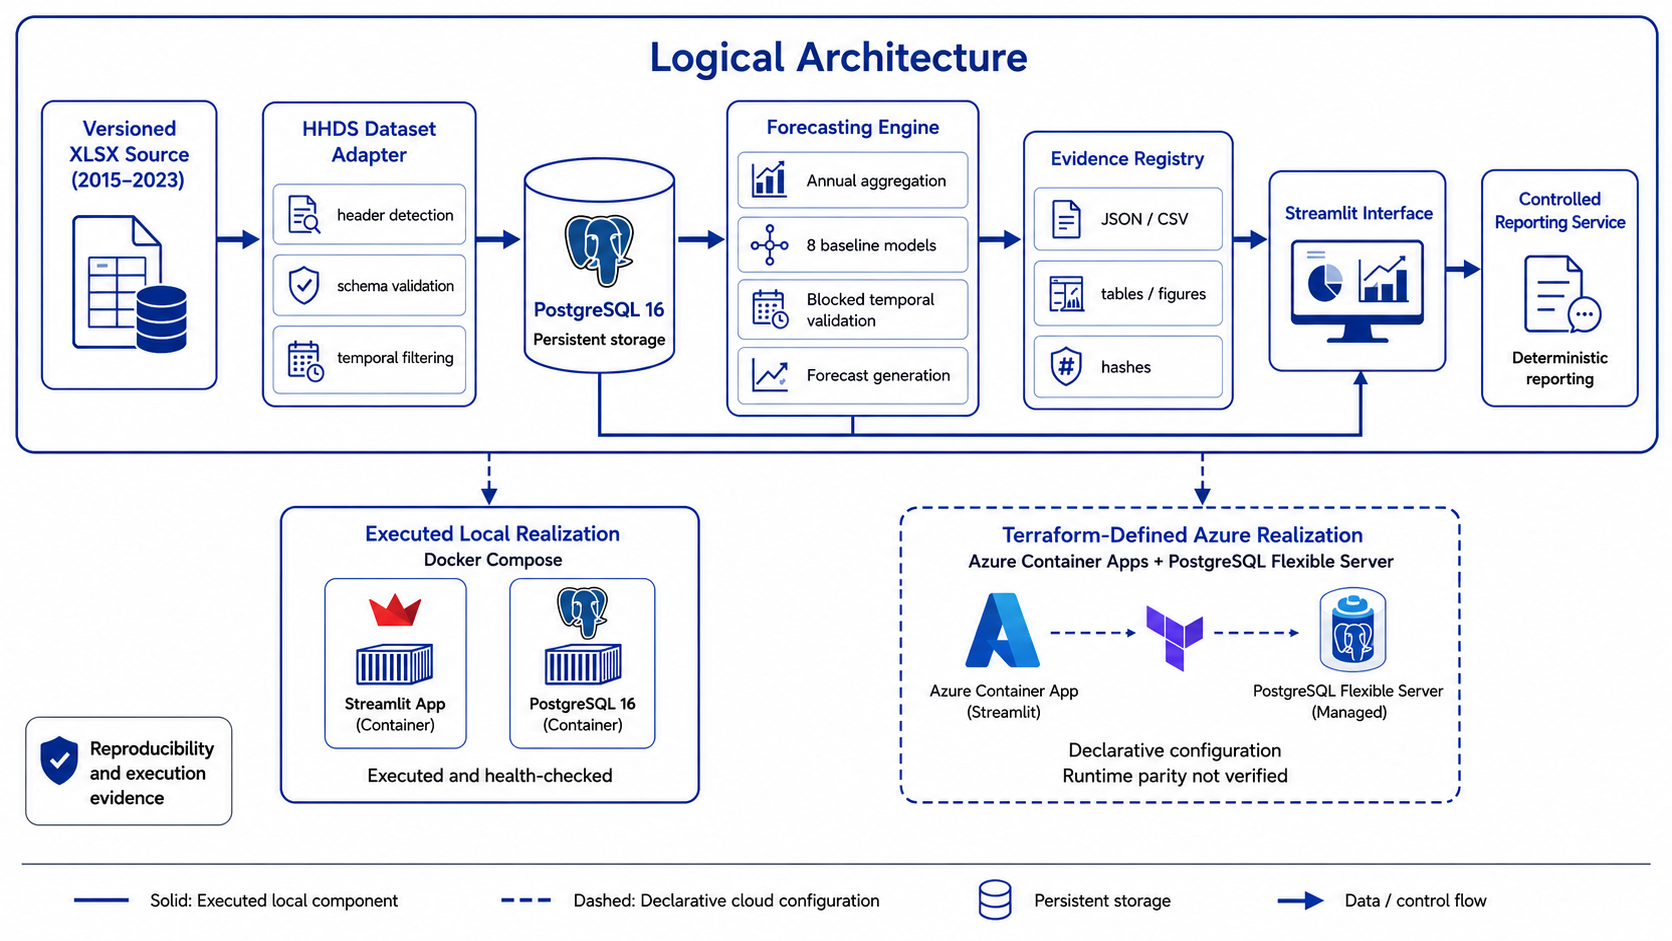
\includegraphics[width=\linewidth,height=0.35\textheight,keepaspectratio]{fig2.png}
                \caption{Logical architecture and physical realizations. Solid borders denote executed local components; dashed borders denote Terraform-defined Azure resources whose runtime parity was not evaluated.}
                \label{fig:architecture}
            \end{figure}

            We drew the workbook from the official SENESCYT open-data repository~\cite{ref13}. A deterministic adapter, HHDS (Heuristic Header Detection and Sanitization), prepares it in a fixed sequence: it scans the first 20 rows, keeps the candidate header whose overlap with the declared schema is highest, drops empty or undeclared fields, checks that every year falls within 2015 to 2023, normalizes the categorical values, records provenance, and writes the clean table into PostgreSQL~16~\cite{ref6,ref14}. The retained fields span four dimensions: temporal, institutional, publication, and disciplinary. Figure~\ref{fig:hhds} lays out this pipeline step by step.

            \begin{figure}[H]
                \centering
                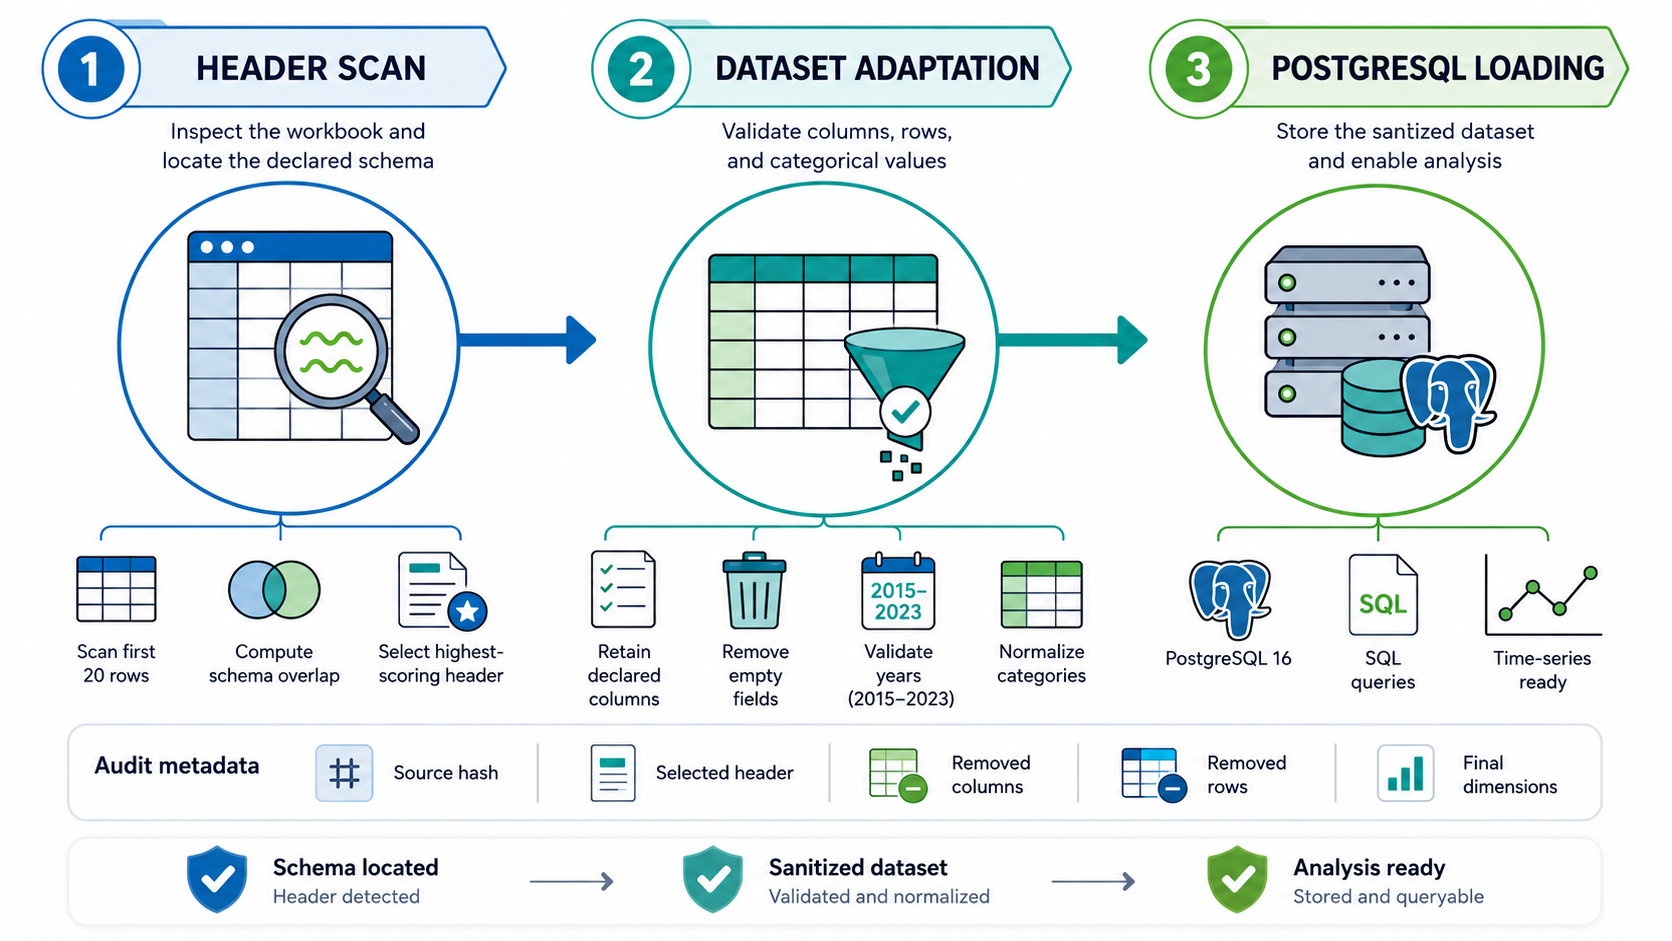
\includegraphics[width=\linewidth,height=0.35\textheight,keepaspectratio]{fig3.png}
                \caption{Deterministic HHDS adaptation: header detection, schema validation, temporal filtering, normalization, provenance capture, and PostgreSQL loading.}
                \label{fig:hhds}
            \end{figure}

            Algorithm~\ref{alg:hhds} states this procedure precisely, from header detection through sanitization to the registration of audit metadata.

            \begin{algorithm}[H]
                \caption{Deterministic Header Detection and Dataset Sanitization}
                \label{alg:hhds}
                \begin{algorithmic}[1]
                    \Require Workbook $D$, declared schema $C^\star$, scan depth $N=20$, valid years $[2015,2023]$
                    \Ensure Sanitized dataset $D_s$ and audit metadata
                    \For{$i=1$ to $N$}
                    \State Normalize candidate row $r_i$ and compute its overlap with $C^\star$
                    \EndFor
                    \State Select the earliest row among those with maximum schema overlap as the header
                    \State Remove preceding rows, unnamed columns, and empty rows
                    \State Retain declared fields and validate the year attribute
                    \State Normalize categorical values and enforce data types
                    \State Record source identity, selected header, removed fields, and row counts
                    \State Load $D_s$ into PostgreSQL~16
                    \State \Return $D_s$ and the registered audit metadata
                \end{algorithmic}
            \end{algorithm}

            Every analytical stage writes to one shared evidence registry, whose contract fixes what must be recorded: the source identity and schema decisions, the fold-level predictions and the selected model, the forecasts and their intervals, and the generated artifacts together with environment metadata, section hashes, and the full scientific payload. Because each value is written once and later read from the same place, the figures, tables, and narrative can no longer disagree with the numbers behind them. Figure~\ref{fig:evidence} follows this evidence from generation through registration to its integrity check.

            \begin{figure}[H]
                \centering
                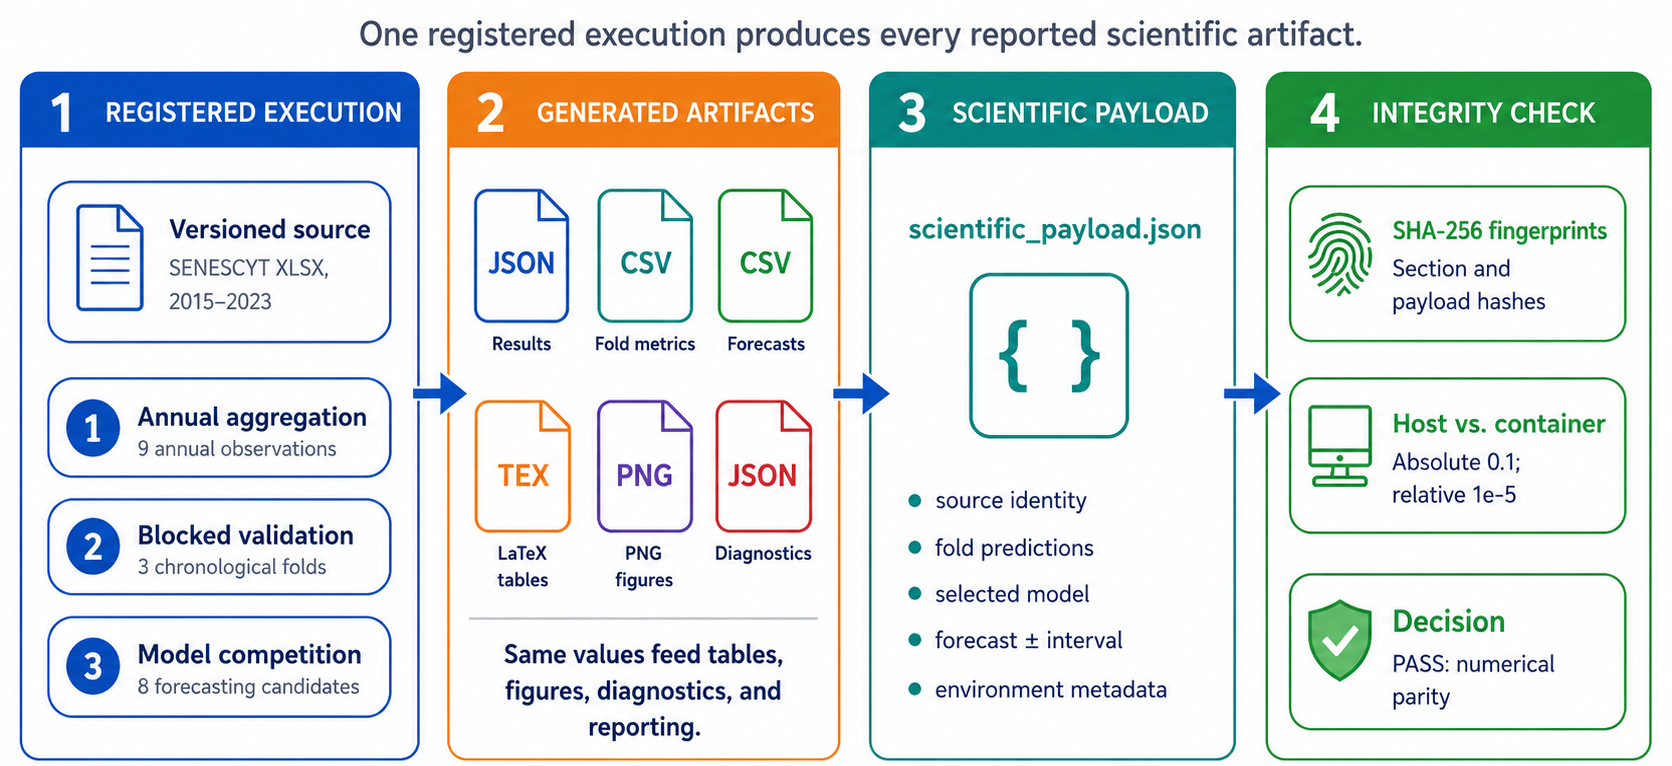
\includegraphics[width=\linewidth,height=0.40\textheight,keepaspectratio]{fig4.png}
                \caption{Auditable evidence generation and integrity checking. Numerical equivalence uses the declared absolute-or-relative rule, while complete hashes preserve the distinction between numerical reproducibility and byte-level identity.}
                \label{fig:evidence}
            \end{figure}

        \subsection{Temporal Evaluation and Forecasting}
            The target is the annual publication count. We compared eight candidates over three blocked folds that keep the years in chronological order~\cite{ref15,ref16,ref17}: Naive, simple exponential smoothing (SES), an automated exponential-smoothing state-space model (ETS), a linear trend, drift, the historical mean, a log-linear trend, and a Poisson generalized linear model (GLM). Equation~(\ref{eq:evaluation}) gives the fold-level mean absolute percentage error (MAPE) together with the instability-adjusted score that drives model selection.

            \begin{equation}
                \mathrm{MAPE}_{m,k}=\frac{100}{n_k}\sum_{t\in V_k}\left|\frac{y_t-\hat y_{m,t}}{y_t}\right|,
                \qquad
                S_\lambda(m)=\overline{\mathrm{MAPE}}_m+\lambda s_m,
                \label{eq:evaluation}
            \end{equation}
            where $s_m$ is the sample standard deviation of the fold MAPE. The main ranking set $\lambda=1$, and we rechecked it at $\lambda\in\{0,0.5,1,2\}$; ties were broken by parsimony, which is a selection rule rather than a claim of statistically significant superiority.

            For the chosen model, six absolute out-of-fold residuals define an exploratory, residual-calibrated interval, written in Eq.~(\ref{eq:interval}).

            \begin{equation}
                PI_{h,0.8}=[\max(0,\hat y_h-q_{0.8}),\,\hat y_h+q_{0.8}],
                \label{eq:interval}
            \end{equation}
            where $q_{0.8}$ is the empirical residual quantile. The idea follows conformal prediction, though a calibration set this small and this dependent cannot promise population-level coverage~\cite{ref18,ref19}. Figure~\ref{fig:model_selection} brings the validation, the candidate comparison, the instability-adjusted ranking, and the final choice of Naive into one view.

            \begin{figure}[H]
                \centering
                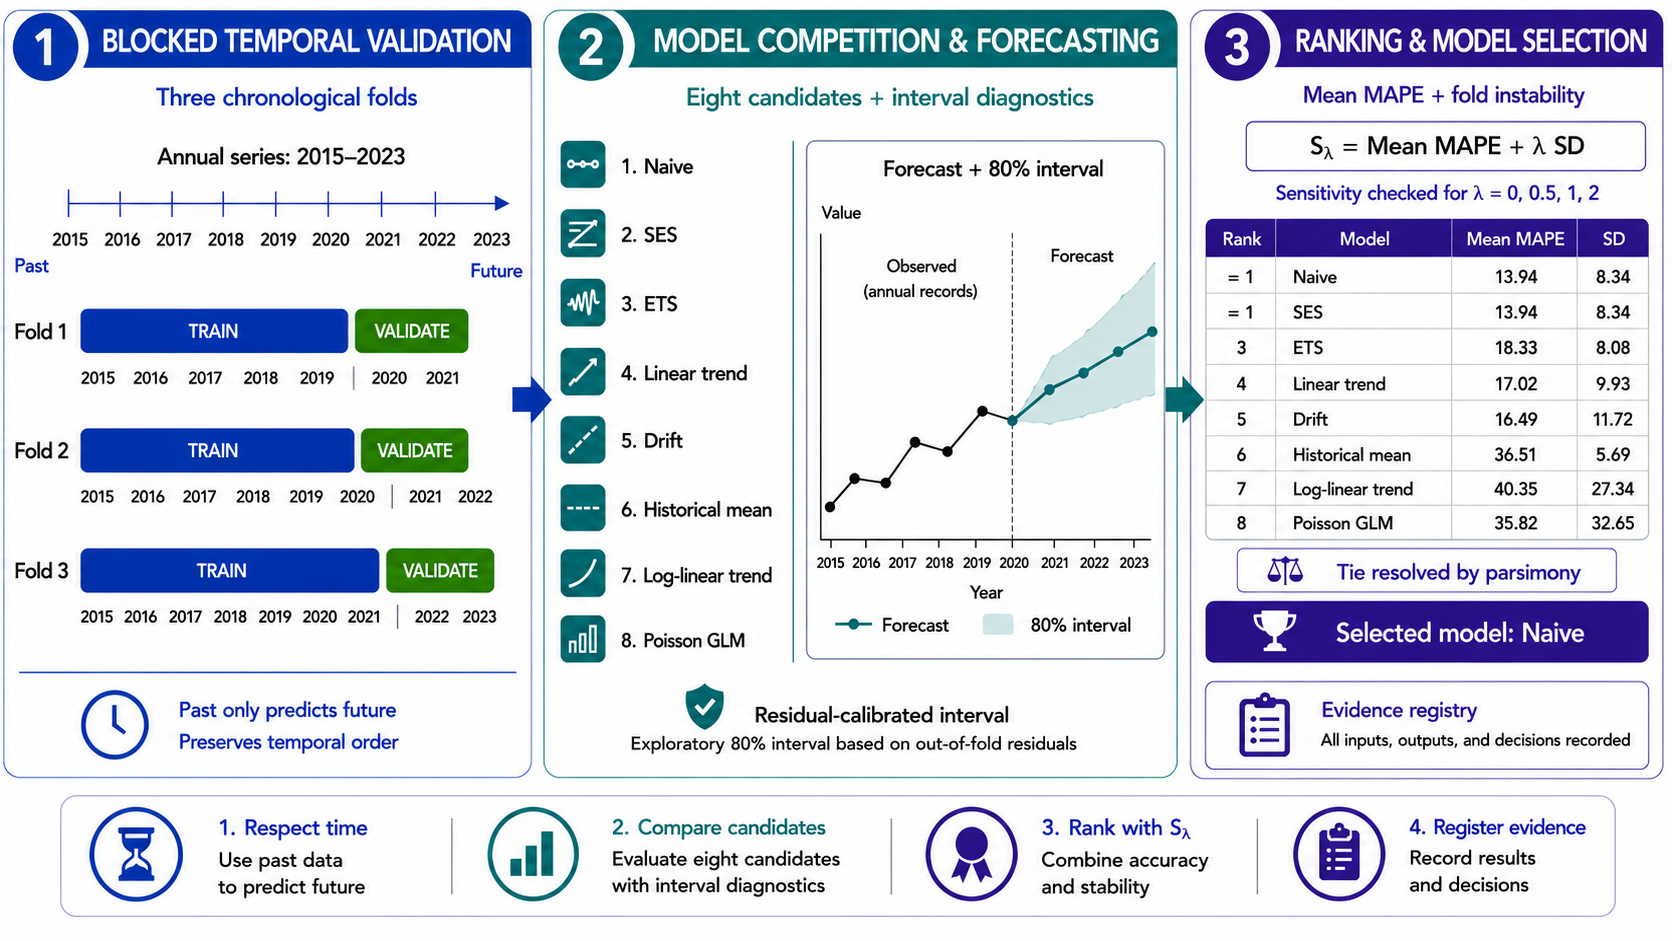
\includegraphics[width=\linewidth,height=0.40\textheight,keepaspectratio]{fig5.png}
                \caption{Blocked temporal validation, comparison of eight forecasting candidates, instability-adjusted ranking, and selection of Naive by parsimony.}
                \label{fig:model_selection}
            \end{figure}

            Algorithm~\ref{alg:temporal_evaluation} sets out the full computation, from temporal evaluation and forecasting to the registration of evidence.

            \begin{algorithm}[H]
                \caption{Blocked Temporal Evaluation and Evidence Registration}
                \label{alg:temporal_evaluation}
                \begin{algorithmic}[1]
                    \Require Annual series $Y$, candidate set $\mathcal{M}$, three chronological folds, horizon $H=\{2024,2025,2026\}$
                    \Ensure Selected model, forecasts, interval, and registered scientific payload
                    \For{each candidate $m\in\mathcal{M}$}
                    \For{each chronological fold $k$}
                    \State Fit $m$ using only observations preceding validation block $V_k$
                    \State Predict $V_k$ and compute $\mathrm{MAPE}_{m,k}$
                    \State Store fold predictions and absolute residuals
                    \EndFor
                    \State Compute mean MAPE, fold SD, and the primary score $S_1(m)$
                    \EndFor
                    \State Select the minimum-score candidate and resolve exact ties by parsimony
                    \State Refit the selected model using the complete annual series
                    \State Generate forecasts for $H$ and the exploratory residual-calibrated interval
                    \State Register folds, metrics, forecasts, figures, diagnostics, and hashes
                    \State \Return the registered scientific payload
                \end{algorithmic}
            \end{algorithm}

        \subsection{Reporting and Reproducibility Protocol}

            The reporting path we evaluated is deterministic and offline: a schema-validated template renders the narrative, tables, and figures straight from the registered payload. A GPT-4o-mini route exists as an option but was left switched off, so we say nothing here about the factuality, usefulness, or stability of large language models~\cite{ref20}.

            We compared host and container runs with complete and section-level SHA-256 fingerprints. Non-numeric values had to match character for character. Two numeric values $a$ and $b$ counted as equal when they satisfied either branch of Eq.~(\ref{eq:tolerance}); the branches are joined by a logical OR, never an AND.

            \begin{equation}
                |a-b|\leq 0.1
                \quad \lor \quad
                \frac{|a-b|}{\max(|a|,|b|)}\leq 10^{-5}.
                \label{eq:tolerance}
            \end{equation}

            In practice, then, an absolute difference of at most 0.1 or a relative difference of at most $10^{-5}$ was enough to treat two outputs as equal. The Linux/WSL2 container exposed eight logical CPUs and about 15.52~GB of memory, with no GPU. Host and container ran Python~3.14.5 and 3.14.6, so the test measures tolerance-based numerical reproducibility, not bitwise reproducibility under an identical stack.

    \section{Results}
        Every result below comes from one frozen execution and its containerized replica. The same pipeline code processed the same SENESCYT workbook on the Windows host and inside the Linux/WSL2 container, and the two environments differ only in operating system and Python patch level. Any divergence between them is therefore attributable to the runtime stack rather than to the inputs, the code path, or the selected model, which is what turns the host--container comparison into a controlled test of numerical reproducibility instead of a test of implementation differences. The host run is the reference, and the numbers, fingerprints, and intervals reported here are the values its evidence registry recorded, not quantities recomputed for presentation.

        \subsection{Execution and Cloud Configuration Evidence}

            Ingestion processed the 87,073 records and distinguished 16,599 raw journal-title strings in 16.44~s, about 5,296 records per second for this one workbook on this one machine; this is a single measurement, not a scalability figure. Figure~\ref{fig:etl} records this extract--transform--load (ETL) run.

            \begin{figure}[!hbt]
                \centering
                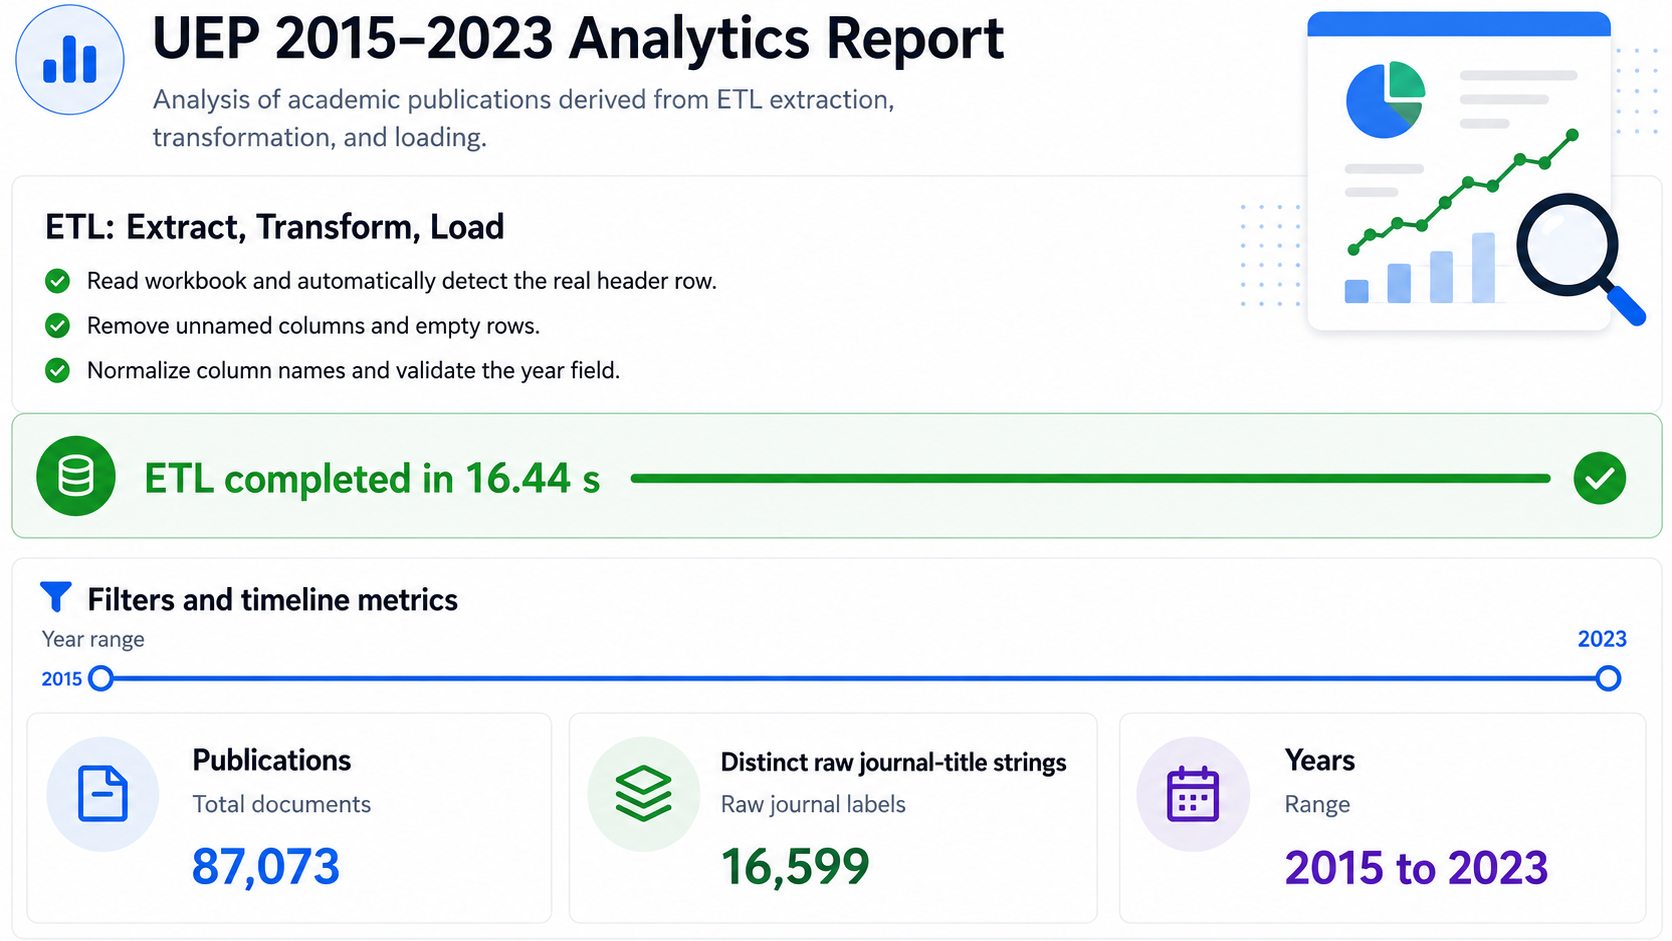
\includegraphics[width=\linewidth,height=0.35\textheight,keepaspectratio]{fig6.png}
                \caption{Extract--transform--load run: 87,073 records and 16,599 distinct raw journal-title strings processed in 16.44~s.}
                \label{fig:etl}
            \end{figure}
            
            The dashboard certifies the deterministic gates behind the counts: header detection, removal of unnamed columns and empty rows, and column-name normalization with year validation. The 87,073 records are therefore a post-sanitization figure with a recorded lineage, not a raw tally, and thus the fixed target the host and container must later reproduce. The 16,599 distinct raw journal-title strings measure the string-level heterogeneity the adapter absorbs, which is why publications are later grouped under normalized labels and why this summary anchors the provenance of the evidence contract rather than reporting performance.
            
            Terraform declares the Azure application, its container environment, the networking, and a managed PostgreSQL instance. This evidence proves that the topology exists as declared, but it stops there: we captured no deployment transcript, health response, cloud payload, successful remote query, timing, or host--Azure comparison. Figure~\ref{fig:azure} shows the declared topology.

            \begin{figure}[H]
                \centering
                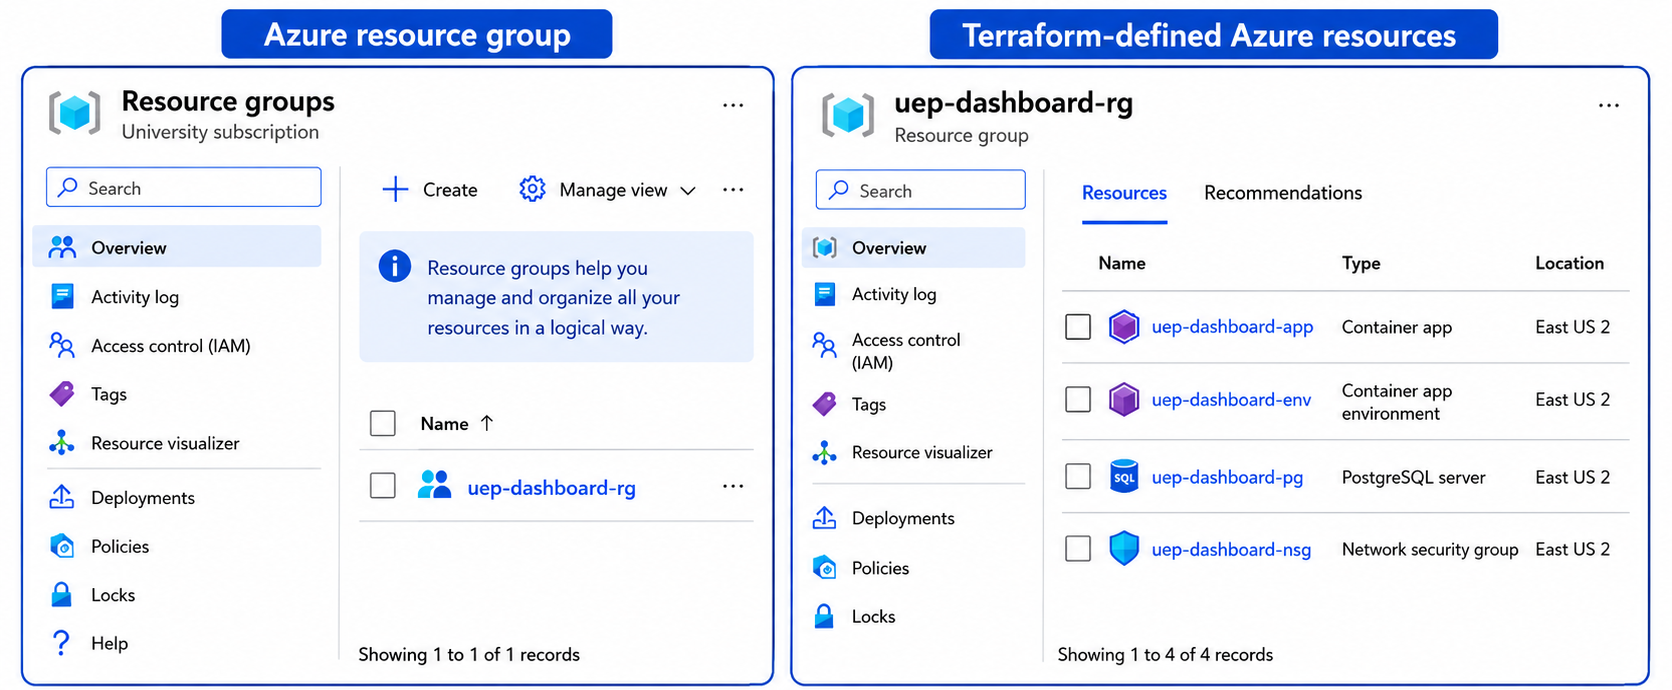
\includegraphics[width=\linewidth,height=0.40\textheight,keepaspectratio]{fig7.png}
                \caption{Terraform-defined Azure resource topology. The figure documents declarative infrastructure, not cloud runtime execution or parity.}
                \label{fig:azure}
            \end{figure}
            
            The resource group makes the local-to-cloud correspondence concrete: its four Terraform-declared members (a Container App, a Container App Environment, a PostgreSQL server, and a Network Security Group) mirror the runtime, database, and network of the evaluated Docker Compose stack. Because they are enumerated from Terraform state rather than created by hand, the topology is reproducible by declaration, since re-applying the same code yields the identical named resources; this is exactly the configuration parity the paper claims and the sense in which the cloud target is auditable without being executed. Yet the claim is bounded: the group certifies a declared topology and network boundary, not a running application, so the security posture shown here is specified but its runtime enforcement remains untested.
            
        \subsection{Host--Container Reproducibility}

            The host ran Windows~11 with Python~3.14.5 and the container ran Linux/WSL2 with Python~3.14.6. Their full payload hashes came out different, but the cause was narrow: 45 small floating-point differences inside the forecasting section, with every non-numeric field identical. Table~\ref{tab:host_container} gathers this evidence.

            \begin{table}[H]
                \caption{Host--container reproducibility evidence.}
                \label{tab:host_container}
                \centering
                \small
                \begin{tabular}{lp{0.60\linewidth}}
                    \toprule
                    \textbf{Evidence} & \textbf{Recorded result} \\
                    \midrule
                    Payload SHA-256 & \begin{tabular}[t]{@{}l@{}}Host: \texttt{ed7198a8bf5d...}\\Container: \texttt{a072859cc944...}\end{tabular} \\
                    Exact parity & No; complete payload fingerprints differ \\
                    Numerical comparison & 45 differences; max. absolute $0.0710614$; max. relative $3.9943\times10^{-5}$ \\
                    Policy and outcome & $|a-b|\leq0.1$ \textbf{OR} relative difference $\leq10^{-5}$; passed. Cases exceeding the relative threshold satisfied the absolute branch \\
                    Scientific output & Naive selected in both; forecasts and intervals agreed under the declared rule \\
                    \bottomrule
                \end{tabular}
            \end{table}

            The reproducibility we can claim, then, is numerical and policy-bound: not byte-level identity, and not Azure runtime parity.

        \subsection{Descriptive and Forecasting Results}
            Annual counts climbed from 3,936 in 2015 to 15,229 in 2023 (3,936, 5,485, 8,611, 9,103, 9,518, 10,326, 11,088, 13,777, and 15,229), though these are administrative records rather than a direct gauge of scientific output. Figure~\ref{fig:heatmap} shows the leading journal labels under English display names, while the counts stay tied to the original raw strings.


            \begin{figure}[H]
                \centering
                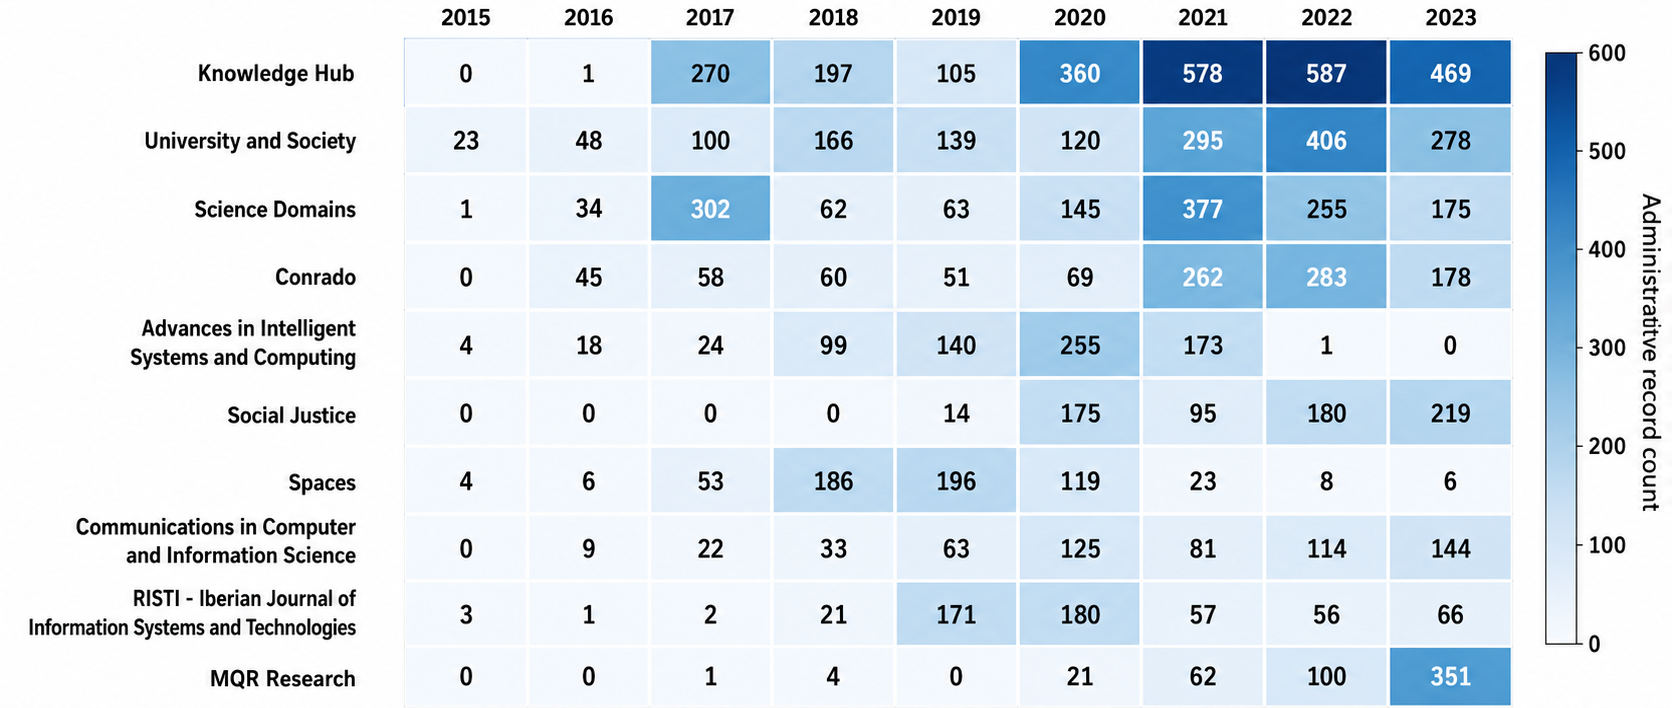
\includegraphics[width=\linewidth,height=0.35\textheight,keepaspectratio]{fig8.png}
                \caption{The ten journal labels with the highest record counts over 2015--2023. Display names are English translations; the counts follow the original raw strings.}
                \label{fig:heatmap}
            \end{figure}

            Naive and SES finished level, at mean MAPE 13.94, fold standard deviation 8.34, and $S_1=22.28$, so parsimony decided the tie in favor of Naive. The Poisson GLM looked strong in the last fold, at 3.5\% MAPE, but swung too widely across the earlier folds to be trusted, and varying $\lambda$ never broke the Naive--SES tie.

            Naive therefore carries the 2023 level forward, projecting 15,229 records for each of 2024, 2025, and 2026, within an exploratory 80\% interval of 9,541.5--20,916.5 (a residual radius of 5,687.5 records). Figure~\ref{fig:forecast} is drawn straight from the registered forecast entries, not recomputed in the reporting layer.

            \begin{figure}[H]
                \centering
                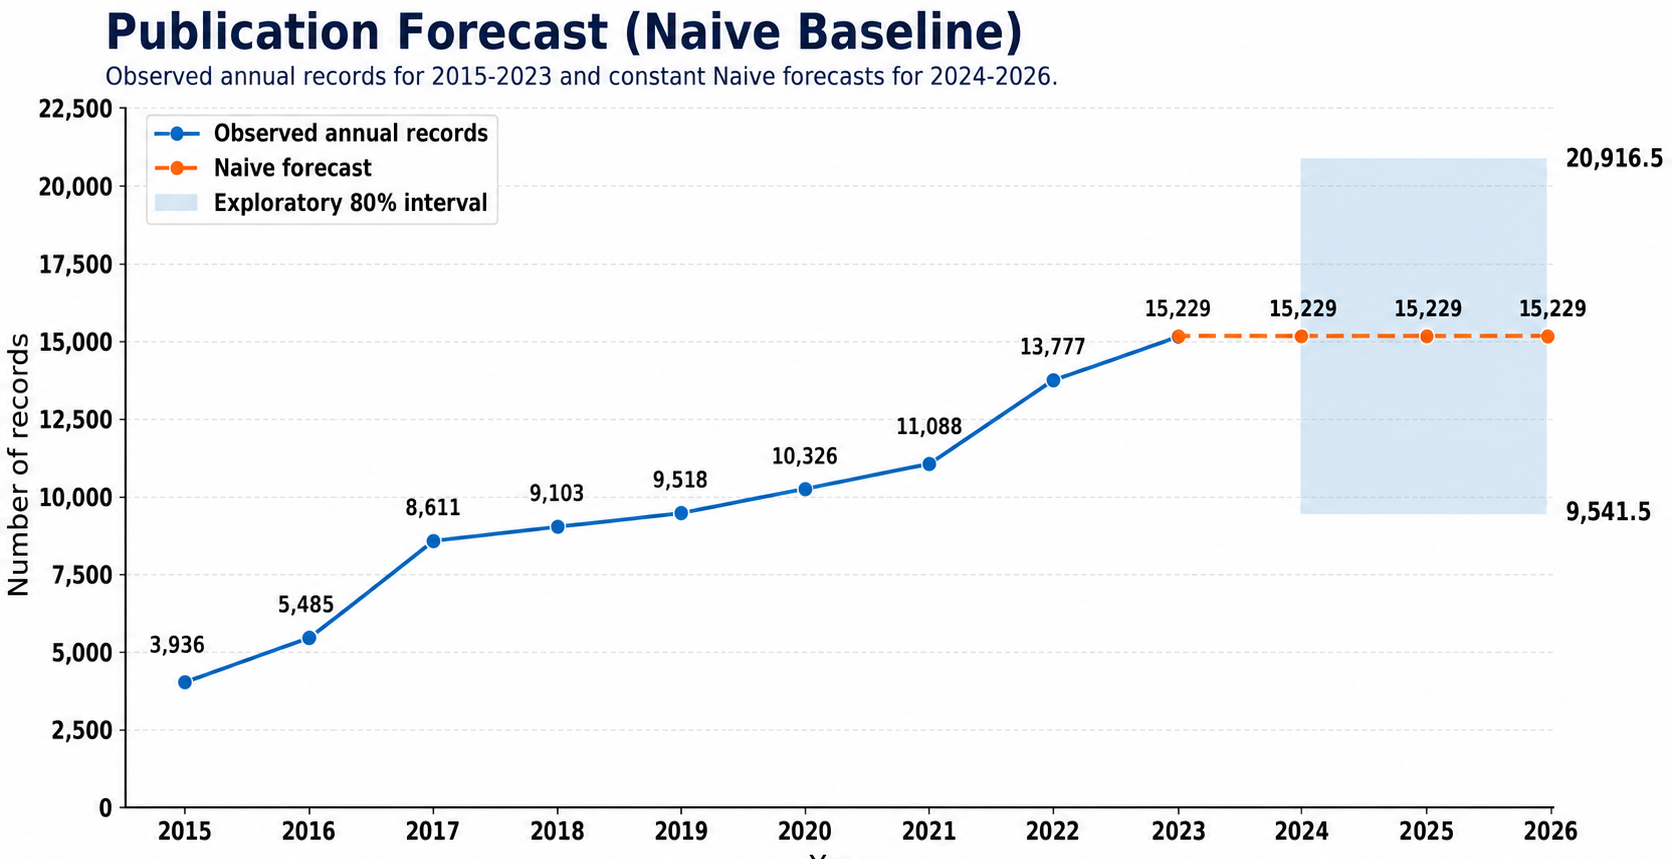
\includegraphics[width=0.9\linewidth,height=0.30\textheight,keepaspectratio]{fig9.png}
                \caption{Observed records and Naive forecasts with an exploratory 80\% interval.}
                \label{fig:forecast}
            \end{figure}

        \subsection{Deterministic Reporting}

            The deterministic reporter reused the same registered forecast, interval, and diagnostics as every other artifact, so the report cannot drift from the analysis behind it. The GPT-4o-mini route was configured but never run, which is why no language-model result appears here. Figure~\ref{fig:reporting} lays out this reporting path.

            \begin{figure}[!hbt]
                \centering
                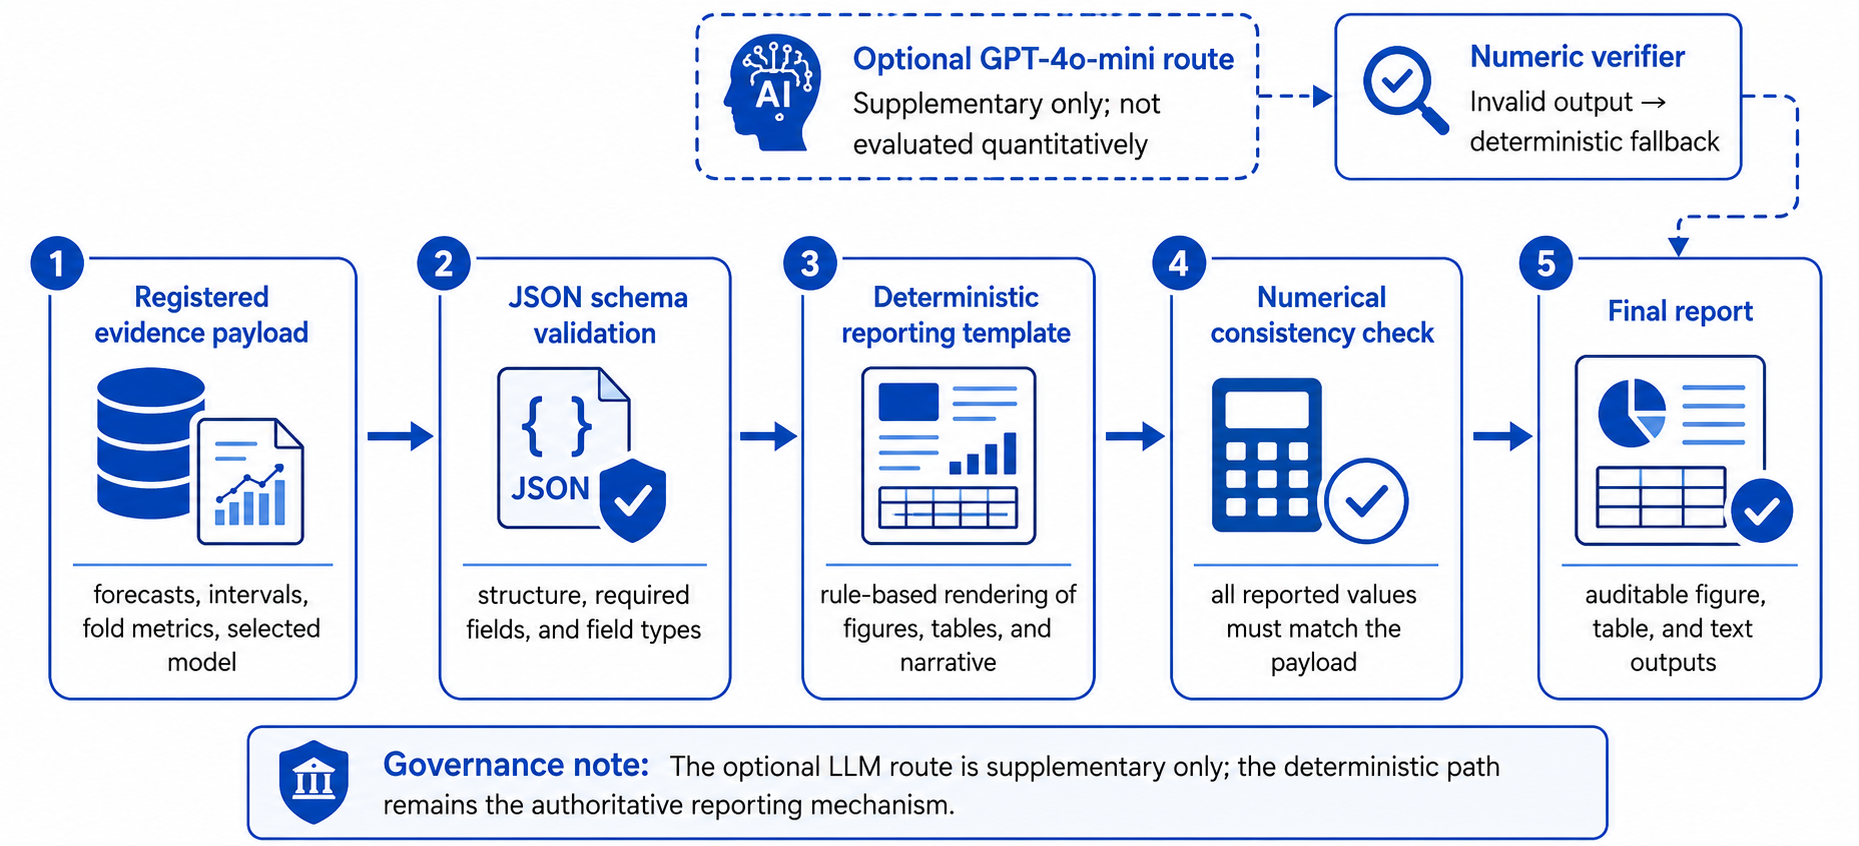
\includegraphics[width=0.9\linewidth,height=0.30\textheight,keepaspectratio]{fig10.png}
                \caption{Reporting workflow. The deterministic route is authoritative; the optional GPT-4o-mini route stays supplementary and unevaluated.}
                \label{fig:reporting}
            \end{figure}

    \section{Discussion}
        Within this bounded case, the three questions have clear answers. The shared registry and its consistent artifacts settle RQ1; the exact match of non-numeric fields, together with the tolerance-level agreement of the 45 numeric differences, settles RQ2; and the exact Naive--SES tie, broken by parsimony, answers RQ3. Where MLOps taxonomies and reviews chart the lifecycle and inventory its components, tools, and stakeholders~\cite{ref2,ref4,ref5,ref14}, and data-centric accounts push data quality and governance to the foreground~\cite{ref24}, they largely stop at prescribing which stages should exist. Our contribution is complementary rather than competing: instead of adding another component to that map, the evidence contract binds the stages that already exist, so that identity, preprocessing, fold predictions, metrics, forecasts, figures, reports, and hashes all trace back to one registered execution and cannot quietly contradict one another.

        This places the work alongside the container- and provenance-based reproducibility literature~\cite{ref7,ref8}, but with a different emphasis. Containers preserve the software environment~\cite{ref7} and provenance-aware engines capture execution records~\cite{ref8}, with recent systems extending capture to end-to-end pipeline provenance~\cite{ref21}; our host--container comparison shows that this preservation is numerical rather than bitwise, since near-identical stacks under Python~3.14.5 and 3.14.6 still produced 45 small floating-point differences. That distance between code availability and identical results is the barrier that surveys of ML reproducibility document~\cite{ref22} and that cross-domain reproducibility frameworks set out to close~\cite{ref25}. Consistent with data-pipeline quality studies that trace downstream errors to schema and provenance failures~\cite{ref6}, the deterministic adapter and the registry are exactly the points where such failures are caught before they reach the manuscript. The declarative-only treatment of Azure keeps this claim honest: unlike cloud-scaling and platform studies that examine runtime behavior~\cite{ref11,ref12}, we claim configuration parity, not execution parity.

        On the forecasting side, the tie between simple baselines and more parameterized models is what the small-sample and temporal-validation literature would anticipate. With nine annual points and three blocked folds, blocked temporal validation is the defensible protocol~\cite{ref15,ref16}, and results on model selection under temporal distribution shift caution against reading a single strong fold as durable evidence~\cite{ref17}; the Poisson GLM, strong in the final fold yet unstable earlier, is a clear instance. The exploratory interval follows conformal principles~\cite{ref18,ref19}, but we deliberately stop short of a coverage guarantee because the calibration set is small and non-exchangeable, precisely the regime those works flag. Simple baselines are therefore more defensible than parameterized rivals here, and the wide interval is the honest price of a short series rather than a defect of the workflow.

        Reproducibility in our setting holds under an explicit tolerance rather than as exact binary identity, and the mismatched Python patch versions are a self-imposed limitation that a stricter replication should remove. Read against work on trustworthy and well-governed AI pipelines~\cite{ref20,ref23,ref26}, the evidence contract operationalizes a narrow but auditable slice of that agenda: it records what was run and lets a third party recompute it, yet it does not yet address continuous training, drift, reliability, security, cost, or cloud scalability.

        Construct validity is bounded by the outcome variable, since an administrative record count is a proxy for scientific productivity rather than a direct measure. Statistical-conclusion validity rests on nine observations, three folds, and six calibration residuals, so neither the ranking gaps nor the interval's coverage should travel beyond this case. Internal validity hinges on the frozen adapter, the fold definitions, the pinned dependencies, and the registry, with the host--container comparison allowing small numerical slack by design. External validity reaches one dataset and one host--container pair; Azure ran only as a declaration, and the language-model route stayed off.
    \section{Conclusions}
        Tied together as Infrastructure-as-Code, the workflow turned a scattered sequence of steps (adaptation, temporal evaluation, persistence, evidence, containers, cloud declaration, and reporting) into one execution that can be re-run and audited. Following design-science guidance on transparent and communicable artifacts~\cite{ref9,ref10}, the evidence contract is the core of that artifact: ingestion finished in 16.44~s for the evaluated workbook, and the payoff appeared as consistency, since host and container agreed on every non-numeric field and, on the 45 numeric differences, stayed within the declared tolerance even though their full hashes differed.

        On the forecasting side, the tie between Naive and SES ($S_1=22.28$) and the parsimony rule that resolved it matter less as a performance result than as proof that model selection, forecast, and interval were recorded and reproduced from the same evidence, extending container- and provenance-based reproducibility~\cite{ref7,ref8} with an explicit, auditable contract. Read against governance frameworks for AI pipelines~\cite{ref20}, the clear next steps are to execute and measure the Azure deployment in full and to replicate the workflow on an independent domain, adding the continuous-training and drift monitoring this version leaves out.

%\subsubsection*{Acknowledgments.}

%%%%%%%%%%%%%%%%%%%%%%%%%%%%%%%%%%%%%%%%%%
    \bibliographystyle{unsrt}
    \bibliography{refs}
\end{document}

